%; whizzy chapter
% -initex iniptex -latex platex -format platex -bibtex jbibtex -fmt fmt
% 以上 whizzytex を使用する場合の設定。

%     Kansai Debian Meeting resources
%     Copyright (C) 2007 Takaya Yamashita
%     Thank you for Tokyo Debian Meeting resources

%     This program is free software; you can redistribute it and/or modify
%     it under the terms of the GNU General Public License as published by
%     the Free Software Foundation; either version 2 of the License, or
%     (at your option) any later version.

%     This program is distributed in the hope that it will be useful,
%     but WITHOUT ANY WARRANTY; without even the implied warranty of
%     MERCHANTABILITY or FITNESS FOR A PARTICULAR PURPOSE.  See the
%     GNU General Public License for more details.

%     You should have received a copy of the GNU General Public License
%     along with this program; if not, write to the Free Software
%     Foundation, Inc., 51 Franklin St, Fifth Floor, Boston, MA  02110-1301 USA

%  preview (shell-command (concat "evince " (replace-regexp-in-string "tex$" "pdf"(buffer-file-name)) "&"))
% 画像ファイルを処理するためにはebbを利用してboundingboxを作成。
%(shell-command "cd image200708; ebb *.png")

%%ここからヘッダ開始。

\documentclass[mingoth,a4paper]{jsarticle}
\usepackage{kansaimonthlyreport}
\usepackage[dvipdfmx]{xy}
\usepackage{etex}
\usepackage{ulem}

% 日付を定義する、毎月変わります。
\newcommand{\debmtgyear}{2016}
\newcommand{\debmtgdate}{24}
\newcommand{\debmtgmonth}{4}
\newcommand{\debmtgnumber}{109}

\def\fixme#1{{\color{red}{#1}}}

\begin{document}

\begin{titlepage}

% 毎月変更する部分、本文の末尾も修正することをわすれずに

  第\debmtgnumber{}回 関西 Debian 勉強会資料

  \vspace{2cm}

  \begin{center}
    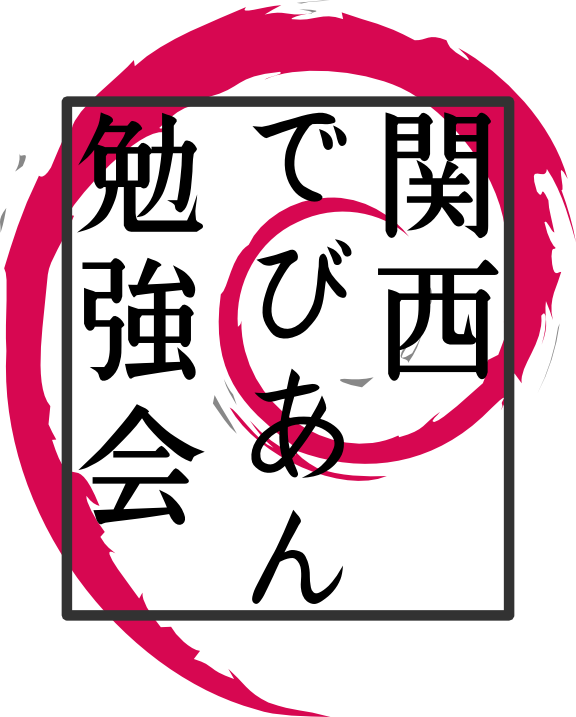
\includegraphics{image200802/kansaidebianlogo.png}
  \end{center}

  \begin{flushright}
    \hfill{}関西Debian勉強会担当者 佐々木・倉敷・のがた・かわだ \\
    \hfill{}\debmtgyear{}年\debmtgmonth{}月\debmtgdate{}日
  \end{flushright}

  \thispagestyle{empty}
\end{titlepage}

\dancersection{Introduction}{Debian JP}

\vspace{1em}

関西Debian勉強会はDebian GNU/Linuxのさまざまなトピック
(新しいパッケージ、Debian特有の機能の仕組、Debian界隈で起こった出来事、
などなど)について話し合う会です。

目的として次の三つを考えています。
\begin{itemize}
\item MLや掲示板ではなく、直接顔を合わせる事での情報交換の促進
\item 定期的に集まれる場所
\item 資料の作成
\end{itemize}

 それでは、楽しい一時をお過ごしください。

\newpage

\begin{minipage}[b]{0.2\hsize}
  {\rotatebox{90}{\fontsize{80}{80}
{\gt{関西 Debian 勉強会}}}}
\end{minipage}
\begin{minipage}[b]{0.8\hsize}
\hrule
\vspace{2mm}
\hrule
\setcounter{tocdepth}{1}
\tableofcontents
\vspace{2mm}
\hrule
\end{minipage}

\dancersection{最近のDebian関係のイベント報告}{Debian JP}

\subsection{第108回関西Debian勉強会}

108回目の関西Debian勉強会は3月27日(日)に福島区民センターで開催されました。

佐々木さんによる「systemdに浸ってみた」でした。

systemd-{timesyncd,resolved,networkd,cron}についてのおはなしでした。次々と新機能
が追加されるsystemd。すべてがSになる。

\subsection{Debian Project}

\subsubsection{Debian Project Leader Election 2016 Results}

2016年度のDebianプロジェクトリーダー選挙が行なわれ、Mehdi Dogguyさんがリーダに選出されました%
\footnote{\url{https://www.debian.org/vote/2016/vote_001}}。

おめでとう、Mehdi Dogguyさん。

\subsubsection{Updated Debian \{7: 7.10, 8: 8.4\} released}

old stable ``wheezy''%
\footnote{\url{https://lists.debian.org/debian-announce/2016/msg00003.html}}
と、stable ``jessie''%
\footnote{\url{https://lists.debian.org/debian-announce/2016/msg00004.html}}
のアップデートがリリースされました。

old stable ``wheezy''のサポートはまもなく終了しますのでまだの方はすみやかに
stable ``jessie''に移行しましょう。

\subsubsection {xscreensaver: please disable "This version of XScreenSaver is very old! Please upgrade!" message}

\debianbug{819703}でxscreensaverが先のメッセージを表示するようになったとのバグが
報告されました。

アップストリームが古いバージョンを使い続けられることを避けるための機能だったので
すが、挙動を変えるということでDebianパッケージでは機能が無効化されました。

やりとりの中でアップストリームから意向を尊重してくれということがあった%
\footnote{\url{https://sources.debian.net/src/xscreensaver/5.34-2/driver/prefs.c/\#L1664}}
のですが、丸くおさまったとはいかなかったようです。

vdirsyncerパッケージでも似たような話し\debianbug{745027}があったようで、
debian-develに「Packages without long term stable releases%
\footnote{\url{https://lists.debian.org/debian-devel/2016/04/msg00054.html}}」
という話題があがっていました。

\subsubsection{debhelper compat 10 ready for testing (debhelper/9.20160403)}

debバイナリパッケージを作成する際に使用する\texttt{debian/rules}ファイルのヘルパー
プログラムであるdebhelperの互換性レベル10がtestingで使えるようになりました%
\footnote{\url{https://lists.debian.org/debian-devel/2016/04/msg00018.html}}。

dh\_installinitは\texttt{ debian/*package* }ファイルをinitスクリプトとしてインストール
しなくなった、など互換性レベル9から11点の変更点があげられています。詳しくは参照元
のメールやchangelogを参照してください。

今後は
\begin{commandline}
$ echo 10 > debian/compat
\end{commandline}
%$
ですね。

\subsubsection{その他}
「Overall bitrot, package reviews and fast(er) unmaintained package removals%
\footnote{\url{https://lists.debian.org/debian-devel/2016/04/msg00076.html}}」
と、腐ってメンテナンスされていないパッケージを速やかに取り除きたいという話題。
debian-devel定期ですね。

「Time for a .changes file format 2.0?%
\footnote{\url{https://lists.debian.org/debian-devel/2016/04/msg00326.html}}」
と、.changeファイルフォーマットを2.0に変更するときではないかという話題。変更点は
wiki:ChangesFormat2.0%
\footnote{\url{https://wiki.debian.org/Teams/Dpkg/Spec/ChangesFormat2.0}}
にまとまっています。


\dancersection{事前課題}{関西Debian勉強会}

今回の課題は以下の通りです。
\begin{screen}
  \begin{enumerate}
  \item %
    ENIAC が作成された目的は何でしょうか?

    調べてみてください。
  \end{enumerate}
\end{screen}

参加者の皆さんの解答は以下の通りです:

\begin{prework}{ むんくさん }
  \begin{enumerate}
  \item かなり以前に雑誌の記事で読んだ記憶では、砲弾の弾道計算のため、だったと思
    います。
  \end{enumerate}
\end{prework}

\begin{prework}{ t3rkwd }
  \begin{enumerate}
  \item 弾道計算。大砲の弾道表をはやく作成するため。
  \end{enumerate}
\end{prework}

\begin{prework}{ murase\_syuka }
  \begin{enumerate}
  \item 大砲の弾道計算
  \end{enumerate}
\end{prework}

\begin{prework}{ Yosuke OTSUKI }
  \begin{enumerate}
  \item 出題者なので、ここでネタばらしはしません。
  \end{enumerate}
\end{prework}

\begin{prework}{ 佐々木洋平 }
  \begin{enumerate}
  \item 当初の目的は「弾道計算」ですよね、フォン・ノイマンの\sout{せい}おかげで、
    最初に計算されたのはマンハッタン計画用の原爆に関する計算だった様ですが。

    自分の専門分野に関係することとして、ENIAC では単純化した系(1層の順圧渦度方程
    式)を問いて「天気予報」が行なわれています。
    こっちは割と詳しく知っていますが、あいにくと弾道計算と原爆関連の計算について
    の詳細は知りません(知ってたら教えて下さい).
  \end{enumerate}
\end{prework}

\begin{prework}{ 川江 浩 }
  \begin{enumerate}
  \item ENIAC(エニアック、Electronic Numerical Integrator and Computer)は、
    アメリカで開発された黎明期の電子計算機(コンピュータ)。チューリング完
    全でディジタル式だがプログラム内蔵方式とするにはプログラムのためのメモ
    リがごくわずかで、パッチパネルによるプログラミングは煩雑ではあったもの
    の、必ずしも専用計算機ではなく広範囲の計算問題を解くことができた
    by Wikipedia
  \end{enumerate}
\end{prework}

\begin{prework}{ Hideo Ueno }
  \begin{enumerate}
  \item アメリカ陸軍の弾道計算用に作られた。真空管で構成されていて完全にデジタ
    ル方式でプログラムが実行された。プログラムはパネルで配線することで行わ
    れ、プログラムの変更の際には、手作業にて配線をやり直す必要があった。

    余談だが、IBMのシステム360が企業に出回るまでは、パンチカードの処理
    を行うために似たような配線式のシステムを使用していたと記憶している。
    (当時はまだ入社下手で、先輩の話を聞いただけで、動かない実物を一度見た
    記憶はあります)
  \end{enumerate}
\end{prework}

\begin{prework}{ hiroshi morimoto }
  \begin{enumerate}
  \item 軍事用に開発されたのでは?。
  \end{enumerate}
\end{prework}


\dancersection{OpenFOAM で数値流体解析}{Yosuke Otsuki}

\subsection{背景: 仕事で数値計算}
飛行機の翼が発生する揚力、建物の耐震性、新薬の成分などは先人たちの発見してくれた
数学的な法則によって、ある程度は計算によって導くことができます。
今日では、これらの方程式を人間が手で解くことは少なくなりつつあります。
数値計算と呼ばれる、人間が方程式を計算機で計算できる形に変形し、実装して、計算機
に解かせる方法にが広がってきたためです。
流体や構造と行った方程式をすでにプログラムしておいて、設計者が数値を入力するだけ
で使えるようになっているソフトウェアを使用し工学に応用することを CAE (Computer
Aided Engineering)といいます。

CAEは主に3つの分野に分類できます。
解析する形状を作成する (CAD)、解析を行う (ソルバー)、そして、解析の結果を確認する
(可視化) の3分野です。
本日紹介する OpenFOAM は、流体分野に特化した解析を行うソフトです。

\subsection{概要: なぜOpen Sourceの解析ソフト ? }
数値計算は多くの計算資源を必要とします。
ハードウェアが安価になったことから、複数ノードによる分散処理によって大規模な問題
を解く方法が一般的に広まってきました。
しかし、大抵の場合、商用のCAEソフトウェアはノード単位でライセンスを購入する必要
があり、たとえ計算資源が十分でも金銭的な余裕がなければ、並列計算を利用した解析を
実行できないことがあります。
このような問題から、Opensource の解析ソフトが注目されるようになりました。
実際に製造業の分野での使用も広がっています。
また、商用のソフトとの違いは、拡張性に富んでいることです。
メッシュ関連のライブラリ、乱流モデルのライブラリ、移流行離散化方法のライブラリな
どが用意されており、既存のアプリケーションもそれらのライブラリを呼び出した数百行
程度のソースコードで書かれています。

\subsection{Install}

\subsubsection{Debian}
debian では freefoam というパッケージ名でビルド済みの OpenFOAM を使用することが
できます。
freefoam と OpenFOAM との違いは、freefoam では、kiva%
\footnote{内燃機関に特化した商用解析ソフト}のピストンモデルなどがなく、商用可視化
ソフトへの出力形式なども削られているようです。
OpenFOAM の開発は続けられていますが、freefoam の開発は数年前から止まったままのよ
うです。

\subsubsection{Build: ビルドの準備}
freefoam は debian 系のパッケージならば、お手軽に OpenFOAM を体験できる点で有利で
すが、最新のOpenFOAMには新機能や不具合の修正なども反映されているため、最新版を使
用することをおすすめします。
最新の安定版は、\url{http://www.openfoam.com}からダウンロードできます。
開発版は github のレポジトリを参照してください。\url{https://github.com/OpenFOAM}
ダウンロードするべきアーカイブは 2 つあります。

\begin{commandline}
OpenFOAM-x.y.z.tgz
ThirdParty-x.y.z.tgz
\end{commandline}

OpenFOAM 自体のソースコードと OpenFOAM が必要とするライブラリをまとめたものです。
このライブラリ群は debian のものを使用することもできます。
ただし、OpenFOAM に同梱されたものを使用したほうが、バージョンの互換性が取れるため
安全です。
OpenFOAM が必要とするライブラリのうち ThirdParty にソースが同伴されているものは以
下です。

\begin{commandline}
ThirdParty-x.y.z
 |-- openmpi
 |-- scotch
 |-- pscotch
 |-- metis (option)
 |-- libcgal
\end{commandline}

openmpi は Message Passing Interface のライブラリです。
scotch は領域分割ツール、ptscotch は scotch の並列計算版です。
metis も領域分割ツールです。
libcgal は計算機科学ライブラリです。ドロネー分割機能が依存しています。この機能が
必要なければ、インストールしなくても問題ありません。
boost がバージョン3.0から必要になりました。
ビルドを開始する前に必要なパッケージをインストールしておきます。

\begin{commandline}
sudo apt-get install build-essential flex bison \
	cmake zlib1g-dev libboost-system-dev \
	libboost-thread-dev libopenmpi-dev openmpi-bin \
	gnuplot libreadline-dev libncurses-dev libxt-dev
\end{commandline}

以上で、ビルド環境が整いました。
さらに詳しいシステム要件、どのパッケージをビルドするのに何が依存しているか、
redhat 系での環境構築方法などは、本家のサイトを参照してください。
\url{http://www.openfoam.com/documentation/system-requirements.php}

\subsubsection{Build: ビルド作業}
インストール用のディレクトリを作成してください。ビルド作業もこのディレクトリの中
で行われます。
このディレクトリの場所は必須ではありませんが、これ以外のディレクトリにする場合、
設定ファイルの編集が必要になります。

\begin{commandline}
$ mkdir $HOME/OpenFOAM
\end{commandline}

上記のディレクトリの中で、ソースコードを展開します。
以下、バージョンを3.0.xとします。

\begin{commandline}
$ tar xzf OpenFOAM-3.0.x.tgz
$ tar xzf ThirdParty-3.0.x.tgz
\end{commandline}

設定ファイルは以下です。\verb|$HOME/OpenFOAM| をインストール先にしていない場合は、
これらのファイルの編集をしてください。
また、時間短縮のため、平行コンパイルをおすすめします。
使用する設定ファイルをテキストエディタで開いて、\verb|WM_NCOMPPROCS=4| (\verb|set WM_NCOMPPROCS=4|)
と記述しておくと4並行でコンパイルしてくれます。

\begin{commandline}
$HOME/OpenFOAM/OpenFOAM-3.0.x/etc/bashrc
$HOME/OpenFOAM/OpenFOAM-3.0.x/etc/cshrc
\end{commandline}

設定が完了したら、ビルドを開始します。
まず、設定した変数を反映し、各種ツールにパスが通ったか確認します。

\begin{commandline}
$ cd $HOME/OpenFOAM/OpenFOAM-3.0.x
$ . etc/bashrc
$ cd $WM_PROJECT_DIR | pwd
/home/yosuke/OpenFOAM/OpenFOAM-3.0.x
\end{commandline}
%$

ビルドしようとしている OpenFOAM のディレクトリが表示されるはずです。問題なければ、
ビルドを始めます。
相当高性能なマシンでも30-40分ぐらいかかります。

\begin{commandline}
wmake >& build.log
\end{commandline}

ログにエラーが出ていなければ、ビルド完了です。
ついでに、解析結果を可視化するためのツールもインストールしておきましょう。
paraview という kitware が作成している並列可視化ツールをインストールします。
debian ならば、下記コマンドで簡単にインストールできます。

\begin{commandline}
# apt-get install paraview
\end{commandline}

\subsection{解析してみる}
チュートリアルを利用して解析を行ってみましょう。
今回は、バイクの周りの空気の流れの解析を行ってみましょう。

\begin{commandline}
cd OpenFOAM-3.0.x/tutorials/incompressible/pisoFoam/les/motoBike/motorBike
ls
0        物理量の初期状態を格納、形状が時間変化する場合は形状情報も格納される
constant 時間変化しない物理量と形状情報を格納
system   各種設定を格納: 空間離散化の方法、時間積分方法、線形ソルバ、領域分割設定、結果出力の時間間隔、時間増分など
\end{commandline}

実際には、このチュートリアルでは、これ以外のファイルがあるはずです。
しかし、これらは簡易実行用のスクリプトやチュートリアル用の初期データなので、解析
には必須ではありません。
必須なのは上記で挙げたディレクトリのみです。

\subsubsection{メッシュの作成}
解析を行うには、1) メッシュを作成, 2) 入力値を設定する, 3) 並列計算する場合は、
領域を分割する, 4) 解析を実行する。
以上のようなステップを踏みます。まずはメッシュから作成しましょう。
OpenFOAM では blockMesh と単純形状のみ作成できるメッシャーと snappyHexMesh という
複雑な形状に対応したメッシャーが利用できます。
他にも、一般的なメッシュ作成ツールから形状を取り込むこともできます。
snappyHexMesh は blockMesh で作成した計算領域を少しずつ形状を変化させ最終形上に近
づけてゆきます。そのため、最初に blockMesh の実行が必要です。

\begin{commandline}
blockMesh

/*---------------------------------------------------------------------------*\
| =========                 |                                                 |
| \\      /  F ield         | OpenFOAM: The Open Source CFD Toolbox           |
|  \\    /   O peration     | Version:  3.0.x                                 |
|   \\  /    A nd           | Web:      www.OpenFOAM.org                      |
|    \\/     M anipulation  |                                                 |
\*---------------------------------------------------------------------------*/
Build  : 3.0.x-c20b114ceb6f
Exec   : blockMesh
Date   : Apr 19 2016
Time   : 00:17:19
Host   : "ca200"
PID    : 4720

.
. 中略
.

  patch 3 (start: 3840 size: 64) name: outlet
  patch 4 (start: 3904 size: 160) name: lowerWall
  patch 5 (start: 4064 size: 160) name: upperWall

End
\end{commandline}

一度 paraview を起動して現在どのようなメッシュが作成されているか観察してみること
にしましょう。
まず、paraview を起動します。

\begin{commandline}
$ paraview &
\end{commandline}
%$

[File] / [Open] から Open File: ダイアログを開きます。 [Files of type] から
[All files (*)] を選択すると、Filename に controlDict というファイルが現れるはず
です。
そのファイルを選択し [OK] ボタンを押し、[Open With] ダイアログのファイル形式のリ
ストから OpenFOAM を選択してください。
[OK] ボタンを押下すると、メインの画面に戻ります。
その後 [Apply] ボタンを押すと
四角いブロックが表示されるはずです。

今度は、snappyHexMesh を使用して実形状のメッシュを作ります。
このメッシャーは、並列実行することが可能です。
\verb|numberOfSubdomains| を編集して 2 にし、そして、\verb|simpleCoeffs| の
\verb|n ( 2 1 1 )| としてあります。
これは、先ほどの四角いブロックを2分割して並列でメッシュ作成を行います。
\verb|n| の成分をすべて乗算したとき、\verb|numberOfSubdomains| と同じになるように
してください。

\begin{commandline}
vi system/decomposeParDict

/*--------------------------------*- C++ -*----------------------------------*\
| =========                 |                                                 |
| \\      /  F ield         | OpenFOAM: The Open Source CFD Toolbox           |
|  \\    /   O peration     | Version:  3.0.x                                 |
|   \\  /    A nd           | Web:      www.OpenFOAM.org                      |
|    \\/     M anipulation  |                                                 |
\*---------------------------------------------------------------------------*/
FoamFile
{
    version     2.0;
    format      ascii;
    class       dictionary;
    location    "system";
    object      decomposeParDict;
}
// * * * * * * * * * * * * * * * * * * * * * * * * * * * * * * * * * * * * * //

numberOfSubdomains 2;

method          ptscotch;

simpleCoeffs
{
    n               (2 1 1);
    delta           0.001;
}

hierarchicalCoeffs
{
    n               (2 1 1);
    delta           0.001;
    order           xyz;
}

manualCoeffs
{
    dataFile        "cellDecomposition";
}


// ************************************************************************* //
\end{commandline}

お使いの計算機のコア数と同じにすると、最も効率よく実行できます。
並列で snappyHexMesh を使用するには下記のように実行します。

\begin{commandline}
mpirun -np 2 snappyHexMesh -parallel >& snappyHexMesh.log
\end{commandline}

計算にはかなり時間がかかります。
先ほどと同じように、paraview で作成したメッシュを見てみましょう。
バイクを運転しているひとのメッシュが作成されているはずです。\\
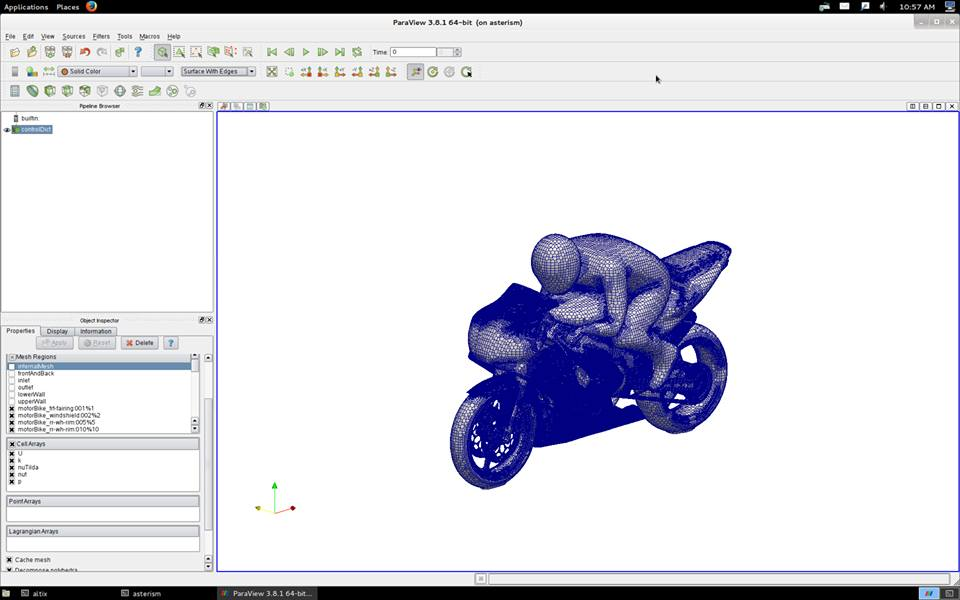
\includegraphics[scale=0.5]{image201604/motorbike_mesh.jpg}

\subsection{解析結果を実行する}
解析を実行してみましょう。
今回のチュートリアルは、非圧縮性の粘性流体を PISO 法で解きます。
このアルゴリズムは、pisoFoam というアプリケーションで利用できます。
移流項の空間離散は 1 次風上差分、拡散項は 2 次精度の中心差分を利用しています。
これらは、\verb|system/fvSchemes| で設定されています。
線形ソルバは AMG 前処理ありの CG 法を使用します。
こちらは、\verb|system/fvSolutions| で設定されています。

\subsection{解析結果を見てみる}
解析は終了しましたが、解析結果はデータファイルとして出力されただけです。
数値ファイルから、数百万点の要素を持つメッシュから空気の流れを読み取ることなどは
ほぼ不可能です。
そのため、解析結果のデータファイルを人間が目で見て理解できるように表示してくれる
可視化ソフトを使用します。
すでにメッシュ作成のところで紹介済みですが、ここでも paraview を使用します。\\
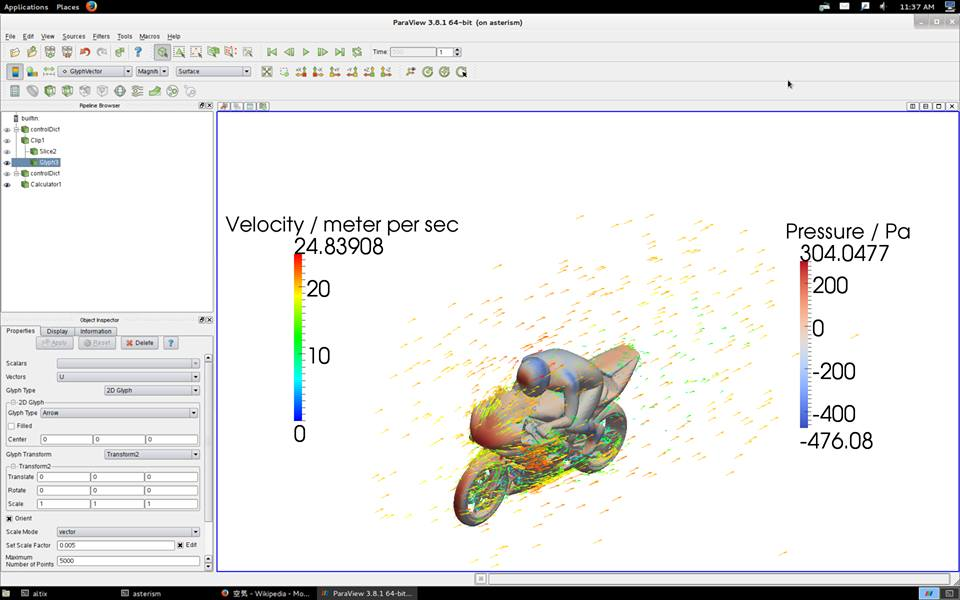
\includegraphics[scale=0.5]{image201604/motorbike_velocity_and_pressure.jpg}

\subsection{まとめ}

\subsubsection{良い点}
OpenFOAMは、商用ソフトと比べて数学的な法則に乗っとてくれているので嬉しいです。商
用のソフトは、数値解析の安定性を確保するために、数学的なトリックを多用しているこ
とが多いです。
1000並列ぐらいまでならば、問題なくスケーリングすることが知られています。ただし、
理論性能比は察してください。
そして、ソースコードさえ読めれば、どんな機能でも自分でカスタマイズなどができるこ
とです。

\subsubsection{悪い点}
数値解析の安定性はあまり良くないです。かなりの数値流体の知識が要求されます。
Unix/Linux に詳しくない技術者にはとっつきにくいかもしれない。


\dancersection{今後の予定}{Debian JP}

\subsection{関西Debian勉強会}
次回、第110回関西Debian勉強会は5月21日(土)か22(日)に開催予定です。
いつもの第4日曜日ではなく土曜日の開催を検討しております。

\subsection{東京エリアDebian勉強会}
次回、第139回東京エリアDebian勉強会は5月21日(土)に開催予定です。

%
% 冊子にするために、4の倍数にする必要がある。
% そのための調整
\dancersection{メモ}{}
\mbox{}\newpage
\mbox{}\newpage
\mbox{}\newpage

\pagebreak

\begin{center}
本資料のライセンスについて
\end{center}

本資料はフリー・ソフトウェアです。あなたは、Free Software
Foundation が公表したGNU GENERAL PUBLIC LICENSEの "バージョン2"もしくはそれ以降
が定める条項に従って本プログラムを再頒布または変更することができ
ます。

本プログラムは有用とは思いますが、頒布にあたっては、市場性及び特
定目的適合性についての暗黙の保証を含めて、いかなる保証も行ないま
せん。詳細についてはGNU GENERAL PUBLIC LICENSE をお読みください。

\begin{multicols}{2}
 \begin{fontsize}{6}{6}
 \begin{verbatim}
            GNU GENERAL PUBLIC LICENSE
               Version 2, June 1991

 Copyright (C) 1989, 1991 Free Software Foundation, Inc.
    51 Franklin St, Fifth Floor, Boston, MA  02110-1301  USA
 Everyone is permitted to copy and distribute verbatim copies
 of this license document, but changing it is not allowed.

                Preamble

  The licenses for most software are designed to take away your
freedom to share and change it.  By contrast, the GNU General Public
License is intended to guarantee your freedom to share and change free
software--to make sure the software is free for all its users.  This
General Public License applies to most of the Free Software
Foundation's software and to any other program whose authors commit to
using it.  (Some other Free Software Foundation software is covered by
the GNU Library General Public License instead.)  You can apply it to
your programs, too.

  When we speak of free software, we are referring to freedom, not
price.  Our General Public Licenses are designed to make sure that you
have the freedom to distribute copies of free software (and charge for
this service if you wish), that you receive source code or can get it
if you want it, that you can change the software or use pieces of it
in new free programs; and that you know you can do these things.

  To protect your rights, we need to make restrictions that forbid
anyone to deny you these rights or to ask you to surrender the rights.
These restrictions translate to certain responsibilities for you if you
distribute copies of the software, or if you modify it.

  For example, if you distribute copies of such a program, whether
gratis or for a fee, you must give the recipients all the rights that
you have.  You must make sure that they, too, receive or can get the
source code.  And you must show them these terms so they know their
rights.

  We protect your rights with two steps: (1) copyright the software, and
(2) offer you this license which gives you legal permission to copy,
distribute and/or modify the software.

  Also, for each author's protection and ours, we want to make certain
that everyone understands that there is no warranty for this free
software.  If the software is modified by someone else and passed on, we
want its recipients to know that what they have is not the original, so
that any problems introduced by others will not reflect on the original
authors' reputations.

  Finally, any free program is threatened constantly by software
patents.  We wish to avoid the danger that redistributors of a free
program will individually obtain patent licenses, in effect making the
program proprietary.  To prevent this, we have made it clear that any
patent must be licensed for everyone's free use or not licensed at all.

  The precise terms and conditions for copying, distribution and
modification follow.

            GNU GENERAL PUBLIC LICENSE
   TERMS AND CONDITIONS FOR COPYING, DISTRIBUTION AND MODIFICATION

  0. This License applies to any program or other work which contains
a notice placed by the copyright holder saying it may be distributed
under the terms of this General Public License.  The "Program", below,
refers to any such program or work, and a "work based on the Program"
means either the Program or any derivative work under copyright law:
that is to say, a work containing the Program or a portion of it,
either verbatim or with modifications and/or translated into another
language.  (Hereinafter, translation is included without limitation in
the term "modification".)  Each licensee is addressed as "you".

Activities other than copying, distribution and modification are not
covered by this License; they are outside its scope.  The act of
running the Program is not restricted, and the output from the Program
is covered only if its contents constitute a work based on the
Program (independent of having been made by running the Program).
Whether that is true depends on what the Program does.

  1. You may copy and distribute verbatim copies of the Program's
source code as you receive it, in any medium, provided that you
conspicuously and appropriately publish on each copy an appropriate
copyright notice and disclaimer of warranty; keep intact all the
notices that refer to this License and to the absence of any warranty;
and give any other recipients of the Program a copy of this License
along with the Program.

You may charge a fee for the physical act of transferring a copy, and
you may at your option offer warranty protection in exchange for a fee.

  2. You may modify your copy or copies of the Program or any portion
of it, thus forming a work based on the Program, and copy and
distribute such modifications or work under the terms of Section 1
above, provided that you also meet all of these conditions:

    a) You must cause the modified files to carry prominent notices
    stating that you changed the files and the date of any change.

    b) You must cause any work that you distribute or publish, that in
    whole or in part contains or is derived from the Program or any
    part thereof, to be licensed as a whole at no charge to all third
    parties under the terms of this License.

    c) If the modified program normally reads commands interactively
    when run, you must cause it, when started running for such
    interactive use in the most ordinary way, to print or display an
    announcement including an appropriate copyright notice and a
    notice that there is no warranty (or else, saying that you provide
    a warranty) and that users may redistribute the program under
    these conditions, and telling the user how to view a copy of this
    License.  (Exception: if the Program itself is interactive but
    does not normally print such an announcement, your work based on
    the Program is not required to print an announcement.)

These requirements apply to the modified work as a whole.  If
identifiable sections of that work are not derived from the Program,
and can be reasonably considered independent and separate works in
themselves, then this License, and its terms, do not apply to those
sections when you distribute them as separate works.  But when you
distribute the same sections as part of a whole which is a work based
on the Program, the distribution of the whole must be on the terms of
this License, whose permissions for other licensees extend to the
entire whole, and thus to each and every part regardless of who wrote it.

Thus, it is not the intent of this section to claim rights or contest
your rights to work written entirely by you; rather, the intent is to
exercise the right to control the distribution of derivative or
collective works based on the Program.

In addition, mere aggregation of another work not based on the Program
with the Program (or with a work based on the Program) on a volume of
a storage or distribution medium does not bring the other work under
the scope of this License.

  3. You may copy and distribute the Program (or a work based on it,
under Section 2) in object code or executable form under the terms of
Sections 1 and 2 above provided that you also do one of the following:

    a) Accompany it with the complete corresponding machine-readable
    source code, which must be distributed under the terms of Sections
    1 and 2 above on a medium customarily used for software interchange; or,

    b) Accompany it with a written offer, valid for at least three
    years, to give any third party, for a charge no more than your
    cost of physically performing source distribution, a complete
    machine-readable copy of the corresponding source code, to be
    distributed under the terms of Sections 1 and 2 above on a medium
    customarily used for software interchange; or,

    c) Accompany it with the information you received as to the offer
    to distribute corresponding source code.  (This alternative is
    allowed only for noncommercial distribution and only if you
    received the program in object code or executable form with such
    an offer, in accord with Subsection b above.)

The source code for a work means the preferred form of the work for
making modifications to it.  For an executable work, complete source
code means all the source code for all modules it contains, plus any
associated interface definition files, plus the scripts used to
control compilation and installation of the executable.  However, as a
special exception, the source code distributed need not include
anything that is normally distributed (in either source or binary
form) with the major components (compiler, kernel, and so on) of the
operating system on which the executable runs, unless that component
itself accompanies the executable.

If distribution of executable or object code is made by offering
access to copy from a designated place, then offering equivalent
access to copy the source code from the same place counts as
distribution of the source code, even though third parties are not
compelled to copy the source along with the object code.

  4. You may not copy, modify, sublicense, or distribute the Program
except as expressly provided under this License.  Any attempt
otherwise to copy, modify, sublicense or distribute the Program is
void, and will automatically terminate your rights under this License.
However, parties who have received copies, or rights, from you under
this License will not have their licenses terminated so long as such
parties remain in full compliance.

  5. You are not required to accept this License, since you have not
signed it.  However, nothing else grants you permission to modify or
distribute the Program or its derivative works.  These actions are
prohibited by law if you do not accept this License.  Therefore, by
modifying or distributing the Program (or any work based on the
Program), you indicate your acceptance of this License to do so, and
all its terms and conditions for copying, distributing or modifying
the Program or works based on it.

  6. Each time you redistribute the Program (or any work based on the
Program), the recipient automatically receives a license from the
original licensor to copy, distribute or modify the Program subject to
these terms and conditions.  You may not impose any further
restrictions on the recipients' exercise of the rights granted herein.
You are not responsible for enforcing compliance by third parties to
this License.

  7. If, as a consequence of a court judgment or allegation of patent
infringement or for any other reason (not limited to patent issues),
conditions are imposed on you (whether by court order, agreement or
otherwise) that contradict the conditions of this License, they do not
excuse you from the conditions of this License.  If you cannot
distribute so as to satisfy simultaneously your obligations under this
License and any other pertinent obligations, then as a consequence you
may not distribute the Program at all.  For example, if a patent
license would not permit royalty-free redistribution of the Program by
all those who receive copies directly or indirectly through you, then
the only way you could satisfy both it and this License would be to
refrain entirely from distribution of the Program.

If any portion of this section is held invalid or unenforceable under
any particular circumstance, the balance of the section is intended to
apply and the section as a whole is intended to apply in other
circumstances.

It is not the purpose of this section to induce you to infringe any
patents or other property right claims or to contest validity of any
such claims; this section has the sole purpose of protecting the
integrity of the free software distribution system, which is
implemented by public license practices.  Many people have made
generous contributions to the wide range of software distributed
through that system in reliance on consistent application of that
system; it is up to the author/donor to decide if he or she is willing
to distribute software through any other system and a licensee cannot
impose that choice.

This section is intended to make thoroughly clear what is believed to
be a consequence of the rest of this License.

  8. If the distribution and/or use of the Program is restricted in
certain countries either by patents or by copyrighted interfaces, the
original copyright holder who places the Program under this License
may add an explicit geographical distribution limitation excluding
those countries, so that distribution is permitted only in or among
countries not thus excluded.  In such case, this License incorporates
the limitation as if written in the body of this License.

  9. The Free Software Foundation may publish revised and/or new versions
of the General Public License from time to time.  Such new versions will
be similar in spirit to the present version, but may differ in detail to
address new problems or concerns.

Each version is given a distinguishing version number.  If the Program
specifies a version number of this License which applies to it and "any
later version", you have the option of following the terms and conditions
either of that version or of any later version published by the Free
Software Foundation.  If the Program does not specify a version number of
this License, you may choose any version ever published by the Free Software
Foundation.

  10. If you wish to incorporate parts of the Program into other free
programs whose distribution conditions are different, write to the author
to ask for permission.  For software which is copyrighted by the Free
Software Foundation, write to the Free Software Foundation; we sometimes
make exceptions for this.  Our decision will be guided by the two goals
of preserving the free status of all derivatives of our free software and
of promoting the sharing and reuse of software generally.

                NO WARRANTY

  11. BECAUSE THE PROGRAM IS LICENSED FREE OF CHARGE, THERE IS NO WARRANTY
FOR THE PROGRAM, TO THE EXTENT PERMITTED BY APPLICABLE LAW.  EXCEPT WHEN
OTHERWISE STATED IN WRITING THE COPYRIGHT HOLDERS AND/OR OTHER PARTIES
PROVIDE THE PROGRAM "AS IS" WITHOUT WARRANTY OF ANY KIND, EITHER EXPRESSED
OR IMPLIED, INCLUDING, BUT NOT LIMITED TO, THE IMPLIED WARRANTIES OF
MERCHANTABILITY AND FITNESS FOR A PARTICULAR PURPOSE.  THE ENTIRE RISK AS
TO THE QUALITY AND PERFORMANCE OF THE PROGRAM IS WITH YOU.  SHOULD THE
PROGRAM PROVE DEFECTIVE, YOU ASSUME THE COST OF ALL NECESSARY SERVICING,
REPAIR OR CORRECTION.

  12. IN NO EVENT UNLESS REQUIRED BY APPLICABLE LAW OR AGREED TO IN WRITING
WILL ANY COPYRIGHT HOLDER, OR ANY OTHER PARTY WHO MAY MODIFY AND/OR
REDISTRIBUTE THE PROGRAM AS PERMITTED ABOVE, BE LIABLE TO YOU FOR DAMAGES,
INCLUDING ANY GENERAL, SPECIAL, INCIDENTAL OR CONSEQUENTIAL DAMAGES ARISING
OUT OF THE USE OR INABILITY TO USE THE PROGRAM (INCLUDING BUT NOT LIMITED
TO LOSS OF DATA OR DATA BEING RENDERED INACCURATE OR LOSSES SUSTAINED BY
YOU OR THIRD PARTIES OR A FAILURE OF THE PROGRAM TO OPERATE WITH ANY OTHER
PROGRAMS), EVEN IF SUCH HOLDER OR OTHER PARTY HAS BEEN ADVISED OF THE
POSSIBILITY OF SUCH DAMAGES.

             END OF TERMS AND CONDITIONS

        How to Apply These Terms to Your New Programs

  If you develop a new program, and you want it to be of the greatest
possible use to the public, the best way to achieve this is to make it
free software which everyone can redistribute and change under these terms.

  To do so, attach the following notices to the program.  It is safest
to attach them to the start of each source file to most effectively
convey the exclusion of warranty; and each file should have at least
the "copyright" line and a pointer to where the full notice is found.

    <one line to give the program's name and a brief idea of what it does.>
    Copyright (C) <year>  <name of author>

    This program is free software; you can redistribute it and/or modify
    it under the terms of the GNU General Public License as published by
    the Free Software Foundation; either version 2 of the License, or
    (at your option) any later version.

    This program is distributed in the hope that it will be useful,
    but WITHOUT ANY WARRANTY; without even the implied warranty of
    MERCHANTABILITY or FITNESS FOR A PARTICULAR PURPOSE.  See the
    GNU General Public License for more details.

    You should have received a copy of the GNU General Public License
    along with this program; if not, write to the Free Software
    Foundation, Inc., 51 Franklin St, Fifth Floor, Boston, MA  02110-1301 USA


Also add information on how to contact you by electronic and paper mail.

If the program is interactive, make it output a short notice like this
when it starts in an interactive mode:

    Gnomovision version 69, Copyright (C) year  name of author
    Gnomovision comes with ABSOLUTELY NO WARRANTY; for details type `show w'.
    This is free software, and you are welcome to redistribute it
    under certain conditions; type `show c' for details.

The hypothetical commands `show w' and `show c' should show the appropriate
parts of the General Public License.  Of course, the commands you use may
be called something other than `show w' and `show c'; they could even be
mouse-clicks or menu items--whatever suits your program.

You should also get your employer (if you work as a programmer) or your
school, if any, to sign a "copyright disclaimer" for the program, if
necessary.  Here is a sample; alter the names:

  Yoyodyne, Inc., hereby disclaims all copyright interest in the program
  `Gnomovision' (which makes passes at compilers) written by James Hacker.

  <signature of Ty Coon>, 1 April 1989
  Ty Coon, President of Vice

This General Public License does not permit incorporating your program into
proprietary programs.  If your program is a subroutine library, you may
consider it more useful to permit linking proprietary applications with the
library.  If this is what you want to do, use the GNU Library General
Public License instead of this License.
 \end{verbatim}
 \end{fontsize}
\end{multicols}

\begin{center}
ソースコードについて
\end{center}

このプログラムは tex で記述されたものです。ソースコードは
\begin{center}
  \url{git://anonscm.debian.org/tokyodebian/monthly-report.git}
\end{center}
から取得できます。

\begin{center}
Debian オープンユーズロゴ ライセンス
\end{center}

\begin{multicols}{2}
 \begin{fontsize}{6}{6}
 \begin{verbatim}

Copyright (c) 1999 Software in the Public Interest
Permission is hereby granted, free of charge, to any person
obtaining a copy of this software and associated documentation
files (the "Software"), to deal in the Software without restriction,
including without limitation the rights to use, copy, modify, merge,
publish, distribute, sublicense, and/or sell copies of the Software,
and to permit persons to whom the Software is furnished to do so,
subject to the following conditions:

The above copyright notice and this permission notice shall be
included in all copies or substantial portions of the Software.

THE SOFTWARE IS PROVIDED "AS IS", WITHOUT WARRANTY OF ANY
KIND, EXPRESS OR IMPLIED, INCLUDING BUT NOT LIMITED TO THE
WARRANTIES OF MERCHANTABILITY, FITNESS FOR A PARTICULAR PURPOSE AND
NONINFRINGEMENT. IN NO EVENT SHALL THE AUTHORS OR COPYRIGHT HOLDERS
BE LIABLE FOR ANY CLAIM, DAMAGES OR OTHER LIABILITY, WHETHER IN
AN ACTION OF CONTRACT, TORT OR OTHERWISE, ARISING FROM, OUT OF OR
IN CONNECTION WITH THE SOFTWARE OR THE USE OR OTHER DEALINGS IN
THE SOFTWARE.
 \end{verbatim}
 \end{fontsize}
\end{multicols}

\printindex
%\cleartooddpage

 \begin{minipage}[b]{0.2\hsize}
  \rotatebox{90}{\fontsize{80}{80} {\gt 関西 Debian 勉強会} }
 \end{minipage}
 \begin{minipage}[b]{0.8\hsize}

 \vspace*{15cm}
 \rule{\hsize}{1mm}
 \vspace{2mm}
 
\includegraphics[width=2cm]{image200502/openlogo-nd.eps}
 \noindent \Large \bfseries{Debian 勉強会資料}\\ \\
 \noindent \normalfont \debmtgyear{}年\debmtgmonth{}月\debmtgdate{}日 \hspace{5mm}  初版第1刷発行\\
 \noindent \normalfont 関西 Debian 勉強会 (編集・印刷・発行)\\
 \rule{\hsize}{1mm}
 \end{minipage}

\end{document}
%%% Local Variables:
%%% skk-kutouten-type: jp
%%% End:
